%%%%%%%%%%%%%%%%%%%%%%%%%%%%%%%%%%%%%%%%%%%%%%%%%%%%%%%%%%%%%%%%%%%%%%%%%%%%
%% Trim Size: 9.75in x 6.5in
%% Text Area: 8in (include Runningheads) x 5in
%% ws-ijseke.tex     22-2-07
%% Tex file to use with ws-ijseke.cls written in Latex2E. 
%% The content, structure, format and layout of this style file is the 
%% property of World Scientific Publishing Co. Pte. Ltd. 
%% Copyright 1995, 2002 by World Scientific Publishing Co. 
%% All rights are reserved.
%%%%%%%%%%%%%%%%%%%%%%%%%%%%%%%%%%%%%%%%%%%%%%%%%%%%%%%%%%%%%%%%%%%%%%%%%%%%
\documentclass{ws-ijseke}

\begin{document}

\markboth{Authors' Names}
{Instructions for Typing Manuscripts (Paper's Title)}

%%%%%%%%%%%%%%%%%%%%% Publisher's Area please ignore %%%%%%%%%%%%%%%
%
\catchline{}{}{}{}{}
%
%%%%%%%%%%%%%%%%%%%%%%%%%%%%%%%%%%%%%%%%%%%%%%%%%%%%%%%%%%%%%%%%%%%%

\title{INSTRUCTIONS FOR TYPESETTING MANUSCRIPTS \\
USING COMPUTER SOFTWARE\footnote{For the title, try not to 
use more than 3 lines. Typeset the title in 10 pt bold and uppercase.}}

\author{FIRST AUTHOR\footnote{
Typeset names in 8 pt Roman, uppercase. Use the footnote to indicate the
present or permanent address of the author.}}

\address{University Department, University Name, Address\\
City, State ZIP/Zone,Country\,\footnote{State completely without 
abbreviations, the affiliation and mailing address, 
including country. Typeset in 8 pt italic.}\\
\email{author\_id@domain\_name\footnote{Typeset author e-mail 
address in single line.}}
\http{$<$webaddress$>$}
}

\author{SECOND AUTHOR}

\address{Group, Laboratory, Address\\
City, State ZIP/Zone, Country\\
author\_id@domain\_name
}

\maketitle

\begin{history}
\received{(Day Month Year)}
\revised{(Day Month Year)}
\accepted{(Day Month Year)}
%\comby{(xxxxxxxxxx)}
\end{history}

\begin{abstract}
The abstract should summarize the context, content and conclusions of
the paper in less than 200 words. It should not contain any reference
citations or displayed equations. Typeset the abstract in 8 pt Roman
with baselineskip of 10 pt, making an indentation of 1.5 pica on the
left and right margins.
\end{abstract}

\keywords{Keyword1; keyword2; keyword3.}

\section{General Appearance \label{ga}}	%) A SECTION HEADING

Contributions to {\it International Journal of Software 
Engineering and Knowledge Engineering} will mostly be processed by
using the authors'source files. These should be submitted with
the manuscripts, and resubmitted in the final form if a paper requires
revision before being accepted for publication.

\section{The Main Text \label{sec1}}
Authors are encouraged to have their contribution checked for grammar. 
American spelling should be used. Abbreviations are
allowed but should be spelt out in full when first used. Integers ten
and below are to be spelt out. Italicize foreign language phrases
(e.g.~Latin, French). Example to cross link for section numbers and 
the main text, Sec.~\ref{sec1}.

The text is to be typeset in 10 pt Roman, single spaced with
baselineskip of 13~pt. Text area (including copyright block) is 
8 inches high and 5 inches wide for the first page.  Text area
(excluding running title) is 7.7 inches high and 5 inches wide for
subsequent pages.  Final pagination and insertion of running titles
will be done by the publisher.

\section{Major Headings}

Major headings should be typeset in boldface with the first letter of
important words capitalized.

\subsection{Sub-headings}

Sub-headings should be typeset in boldface italic and capitalize
the first letter of the first word only. Section number to be in
boldface Roman.

\subsubsection{Sub-subheadings}

Typeset sub-subheadings in medium face italic and capitalize the first
letter of the first word only. Section numbers to be in Roman.

\subsection{Numbering and spacing}

Sections, sub-sections and sub-subsections are numbered in Arabic.
Use double spacing before all section headings, and single spacing
after section headings. Flush left all paragraphs that follow after
section headings.

\subsection{Lists of items}

List may be presented with each item marked by bullets and numbers.

\subsection*{Bulleted items}

\begin{itemlist}
 \item item one,
 \item item two,
 \item item three.
\end{itemlist}

\subsection*{Numbered items}

\begin{arabiclist}
 \item item one,
 \item item two,
 \item item three.
\end{arabiclist}

The order of subdivisions of items in bullet and numbered lists
may be presented as follows:

\subsection*{Bulleted items}

\begin{itemize}
\item First item in the first level
\item Second item in the first level
\begin{itemize}
\item First item in the second level 
\item Second item in the second level
\begin{itemize}
\item First item in the third level 
\item Second item in the third level
\end{itemize}
\item Third item in the second level
\item Fourth item in the second level
\end{itemize}
\item Third item in the first level
\item Fourth item in the first level
\end{itemize}

\subsection*{Numbered items}

\begin{arabiclist}
\item First item in the first level
\item Second item in the first level
\begin{alphlist}[(a)]
\item First item in the second level 
\item Second item in the second level
\begin{romanlist}[iii.]
\item First item in the third level 
\item Second item in the third level
\item Third item in the third level
\end{romanlist}
\item Third item in the second level
\item Fourth item in the second level
\end{alphlist}
\item Third item in the first level
\item Fourth item in the first level
\end{arabiclist}

\section{Equations}

Displayed equations should be numbered consecutively,
with the number set flush right and enclosed in parentheses. The
equation numbers should be consecutive within the contribution.
\begin{equation}
\mu(n, t) = \frac{\sum^\infty_{i=1} 1(d_i < t, N(d_i) = n)}{
\int^t_{\sigma=0} 1(N(\sigma) = n)d\sigma}\, .
\label{eq:jaa}
\end{equation}

Equations should be referred to in abbreviated form,
e.g.~``Eq.~(\ref{eq:jaa})'' or ``(2)''. In multiple-line
equations, the number should be given on the last line.

Displayed equations are to be centered on the page width.
Standard English letters like x are to appear as $x$
(italicized) in the text if they are used as mathematical
symbols. Punctuation marks are used at the end of equations as
if they appeared directly in the text.

\section{Theorem Environments}

\begin{theorem}
Theorems$,$ lemmas$,$ definitions$,$ etc. are set on a separate 
paragraph$,$ with extra 1 line space above and below. They are to 
be numbered consecutively within the contribution.
\end{theorem}

\begin{lemma}
Theorems$,$ lemmas$,$ definitions$,$ etc. are set on a separate 
paragraph$,$ with extra 1 line space above and below. They are to be 
numbered consecutively within the contribution.
\end{lemma}

\begin{proof}
The word `Proof' should be type in boldface. Proofs
should end with\break
a box. 
\end{proof}

\section{Illustrations and Photographs}

\begin{figure}[b]
\centerline{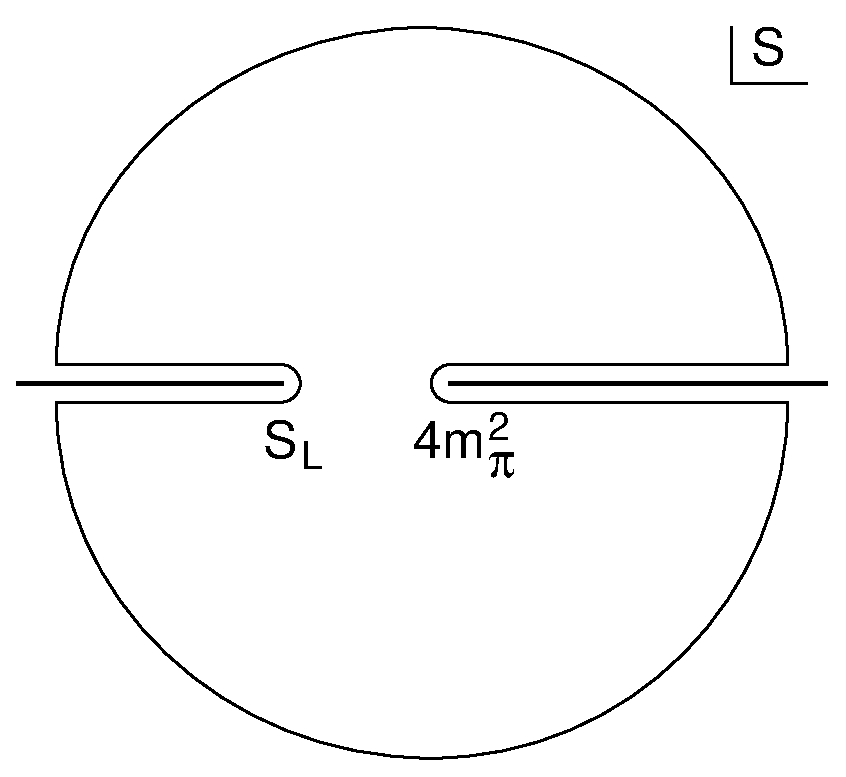
\psfig{file=ijsekef1.eps,width=5cm}}
\vspace*{8pt}
\caption{A schematic illustration of dissociative recombination. The
direct mechanism, 4m$^2_\pi$ is initiated when the
molecular ion S$_{\rm L}$ captures an electron with kinetic energy.}
\end{figure}

Figures are to be inserted in the text nearest their first
reference.  Figure placements can be either top or bottom.
Original india ink drawings of glossy prints are
preferred. Please send one set of originals with copies. If the
author requires the publisher to reduce the figures, ensure that
the figures (including letterings and numbers) are large enough
to be clearly seen after reduction. If photographs are to be
used, only black and white ones are acceptable.

Figures are to be sequentially numbered in Arabic numerals. The
caption must be placed below the figure. Typeset in 8 pt Roman with
baselineskip of 10~pt. Long captions are to be justified by the
``page-width''.  Use double spacing between a caption and the text
that follows immediately.

Previously published material must be accompanied by written
permission from the author and publisher.

\section{Tables}

Tables should be inserted in the text as close to the point of
reference as possible. Some space should be left above and below
the table.

Tables should be numbered sequentially in the text in Arabic
numerals. Captions are to be centralized above the tables.
Typeset tables and captions in 8 pt Roman with
baselineskip of 10 pt. Long captions are to be justified by the ``table-width''.

\begin{table}[h]
\tbl{Comparison of acoustic for frequencies for piston-cylinder problem.}
{\begin{tabular}{@{}cccc@{}} \toprule
Piston mass & Analytical frequency & TRIA6-$S_1$ model &
\% Error \\
& (Rad/s) & (Rad/s) \\ \colrule
1.0\hphantom{00} & \hphantom{0}281.0 & \hphantom{0}280.81 & 0.07 \\
0.1\hphantom{00} & \hphantom{0}876.0 & \hphantom{0}875.74 & 0.03 \\
0.01\hphantom{0} & 2441.0 & 2441.0\hphantom{0} & 0.0\hphantom{0} \\
0.001 & 4130.0 & 4129.3\hphantom{0} & 0.16\\ \botrule
\end{tabular}}
\begin{tabnote}
Table notes.
\end{tabnote}
\begin{tabfootnote}
\tabmark{a} Table footnote A.\\
\tabmark{b} Table footnote B.
\end{tabfootnote}
\end{table}


If tables need to extend over to a second page, the continuation
of the table should be preceded by a caption, 
e.g.~``{\it Table 2.} $(${\it Continued}$)$''. Notes to tables are
placed below the final row of the table and should be flushleft.
Footnotes in tables shouldbe indicated by superscript lowercase letters
and placed beneath the table.


\section{Running Heads}

Please provide a shortened runninghead (not more than eight words) for
the title of your paper. This will appear on the top right-hand side
of your paper.

\section{Footnotes}

Footnotes should be numbered sequentially in superscript
lowercase roman letters.\footnote{Footnotes should be
typeset in 8 pt Roman at the bottom of the page.}

\appendix

\section{Appendices}

Appendices should be used only when absolutely necessary. They
should come before the References. If there is more than one
appendix, number them alphabetically. Number displayed equations
occurring in the Appendix in this way, e.g.~(\ref{appeqn}), (A.2),
etc.
\begin{equation}
\mu(n, t) = \frac{\sum^\infty_{i=1} 1(d_i < t, N(d_i) 
= n)}{\int^t_{\sigma=0} 1(N(\sigma) = n)d\sigma}\,.
\label{appeqn}
\end{equation}

\section*{References}
References are to be listed in the order cited in the text in Arabic 
numerals.  They can be typed after punctuation marks, 
e.g.~``$\ldots$ in the statement \cite{birk}.'' or used directly,
e.g.~``e.g.~``see [\refcite{bergm}] for examples.'' Please list 
using the style shown in the following examples.  For journal names, 
use the standard abbreviations.  Typeset references in 9 pt Roman 
with baselineskip of 11pt.

\section*{Acknowledgements}

This section should come before the References. Funding
information may also be included here.

\begin{thebibliography}{00}

\bibitem{alth} K.-D. Althoff, A. Birk, S. Hartkopf, and W. M\"{u}ller,
Managing software engineering experience for comprehensive reuse, in
{\it Proc.  11th Int. Conf. on Software Engineering}, Kaiserslautern,
Germany, 1999.

\bibitem{birk} K.-D. Althoff, A. Birk, and C. Tautz, The experience 
factory approach: Realizing learning from experience in software 
development organizations, in {\it Proc. 10th German Workshop 
on Machine Learning $($FGML'97$)$}, University of Karlsruhe, 1997, 
pp.~6--8.

\bibitem{basili} V. R. Basili, G. Caldiera, and H. D. Rombach, The
experience factory, in \textit{Encyclopedia of Software Engineering},
ed. J. J. Marciniak,  (John Wiley \& Sons, 1994), pp. 469--476.

\bibitem{romb} V. R. Basili and H. D. Rombach, The TAME project: Towards
improvement-oriented software environments, \textit{IEEE Trans.  on
Software Engineering} {\bf SE-14}(6) (1988) 758--773.

\bibitem{becker} U. Becker-Kornstaedt and R. Webby, A Comprehensive Schema 
Integrating Software Process Modelling and Software Measurement, 
Fraunhofer IESE-Report No. 047.99 (Ed.: Fraunhofer IESE, 1999), 
http://www.iese.fhg.de/Publications/Iese{\_}reports/.

\bibitem{bergm} R. Bergmann and U. Eisenecker, Case-based reasoning for
supporting reuse of object-oriented software: A case study, in {\it
Proc.  Expert Systems} {\bf 95} (1996) 152--169.

\bibitem{ncard} D. N. Card and R. L. Glass, \textit{Measuring Software
Design Quality} (Prentice Hall, Englewood Cliffs, NJ, 1990).

\bibitem{derid} D. Deridder, A concept-oriented approach to support software 
maintenance and reuse activities, in {\it Proc. Workshop on 
Knowledge-Based Object-Oriented Software Engineering at 16th European 
Conference on Object-Oriented Programming $($ECOOP 2002$)$}, M\'{a}laga, 
Spain, 2002.

\bibitem{estay} C. Estay and J. Pastor, Improving action research in
information systems with project management, in {\it Proc. Americas
Conference on Information Systems}, Long Beach, CA, USA, 2000,
pp.~1558--1561.

\bibitem{falbo} R. A. Falbo, C. S. Menezes, and A. R. Rocha, Using
ontologies to improve knowledge integration in software engineering
environments, in {\it Proc. 4th Conference on Information Systems
Analysis and Synthesis}, Orlando, Florida, USA, 1998.
\end{thebibliography}

\end{document}
